\documentclass{IEEEtran}
\usepackage{float}
\usepackage{graphicx}
\usepackage{booktabs}
\renewcommand{\baselinestretch}{1}
\setlength{\textheight}{9in}
\setlength{\textwidth}{6.5in}
\setlength{\headheight}{0in}
\setlength{\headsep}{0in}
\setlength{\topmargin}{0in}
\setlength{\oddsidemargin}{0in}
\setlength{\evensidemargin}{0in}
\setlength{\parindent}{.3in}
\newtheorem{hypothesis}{Hypothesis}
\newtheorem{nullhypothesis}{Null Hypothesis}
\usepackage{gensymb}

\begin{document}
\onecolumn
\section{Mobilenet v3 Training Schedule}

\begin{enumerate}
\item Batch size:150
\item Validation size:50
\item Learning rate 1e-5
\end{enumerate}


\bigskip

EarlyStopping 10 epochs without validation accuracy increasing



\bigskip

\textbf{Mobilenet Conv + Flatten + Softmax Classifier}\newline
CNN non-converging

\bigskip


\bigskip

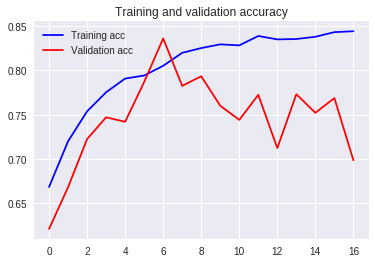
\includegraphics[width=3in,height=2.18in]{mobile/mobilenet-img001.png} 
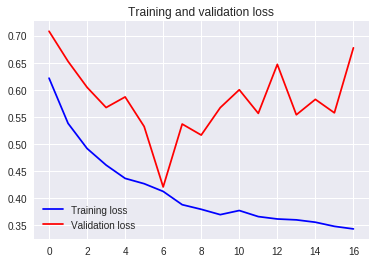
\includegraphics[width=3in,height=2.18in]{mobile/mobilenet-img002.png} 


\bigskip

\begin{table}[htht]
\centering
\caption{Mobilenet Training - Results for Mobilenet + Flatten + Softmax }
\label{mobilenet1}
\begin{tabular}{rcccl}
\textbf{}   & \textbf{Precision} & \textbf{Recall} & \textbf{F1-Score} & \textbf{Support} \\
No Litter   & 0.96 &0.84 & 0.90 & 1172 \\
Litter      & 0.47 &0.82 & 0.60 & 208 \\
avg / total & 0.89 &0.84 & 0.85 & 1380 \\
\end{tabular}
\end{table}

\begin{center}\noindent\rule{10cm}{0.4pt}\end{center}

\bigskip

\textbf{Mobilenet Conv + Global AveragePooling2D + Softmax Classifier}\newline
Accuracy Obtained : 0.8233

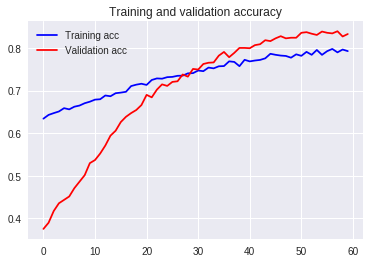
\includegraphics[width=3in,height=2.18in]{mobile/mobilenet-img003.png} 
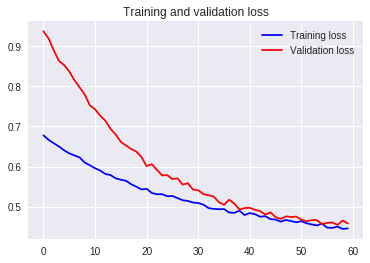
\includegraphics[width=3in,height=2.18in]{mobile/mobilenet-img004.png} 


\bigskip

\begin{table}[ht]
\centering
\caption{Mobilenet Training - Results for Mobilenet + GAP2d + Softmax}
\label{mobilenet1}
\begin{tabular}{rcccl}
\textbf{}   & \textbf{Precision} & \textbf{Recall} & \textbf{F1-Score} & \textbf{Support} \\
No Litter   & 0.95 &0.85 & 0.90 & 1172 \\
Litter      & 0.48 &0.77 & 0.59 & 208 \\
avg / total & 0.88 &0.84 & 0.85 & 1380 \\
\end{tabular}
\begin{center}\noindent\rule{10cm}{0.4pt}\end{center}
\end{table}




\bigskip

\textbf{Mobilenet Conv + Global AveragePooling2D + FCN 1024 width + Softmax Classifier}\newline
Accuracy obtained: 0.84420

 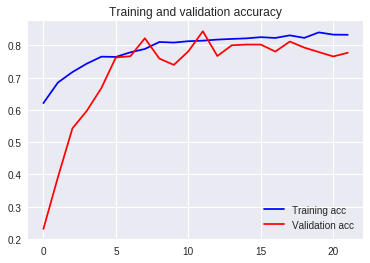
\includegraphics[width=3in,height=2.18in]{mobile/mobilenet-img005.png} 
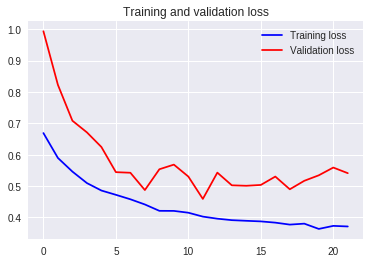
\includegraphics[width=3in,height=2.18in]{mobile/mobilenet-img006.png} 


\bigskip

\begin{table}[ht]
\centering
\caption{Mobilenet Training - Results for Mobilenet + GAP2d + FCN 1024 width + Softmax}
\label{mobilenet1}
\begin{tabular}{rcccl}
\textbf{}   & \textbf{Precision} & \textbf{Recall} & \textbf{F1-Score} & \textbf{Support} \\
No Litter   & 0.98 &0.83 & 0.90 & 1172 \\
Litter      & 0.49 &0.91 & 0.64 & 208 \\
avg / total & 0.91 &0.84 & 0.86 & 1380 \\
\end{tabular}
\begin{center}\noindent\rule{10cm}{0.4pt}\end{center}
\end{table}


\bigskip

\textbf{Mobilenet Conv + Global AveragePooling2D + FCN 2048 width + Softmax Classifier}\newline
Accuracy Obtained: 0.86739

 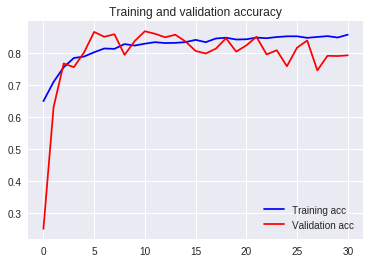
\includegraphics[width=3in,height=2.18in]{mobile/mobilenet-img007.png} 
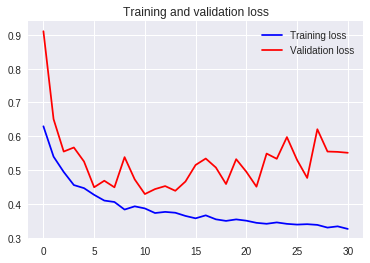
\includegraphics[width=3in,height=2.18in]{mobile/mobilenet-img008.png} 


\bigskip
\begin{table}[ht]
\centering
\caption{Mobilenet Training - Results for Mobilenet + GAP2d + FCN 2048 width + Softmax}
\label{mobilenet1}
\begin{tabular}{rcccl}
\textbf{}   & \textbf{Precision} & \textbf{Recall} & \textbf{F1-Score} & \textbf{Support} \\
No Litter   & 0.98 &0.86 & 0.92 & 1172 \\
Litter      & 0.54 &0.90 & 0.67 & 208 \\
avg / total & 0.91 &0.87 & 0.88 & 1380 \\
\end{tabular}
\begin{center}\noindent\rule{10cm}{0.4pt}\end{center}
\end{table}

\bigskip

\textbf{Mobilenet Conv + Global AveragePooling2D + FCN 4096 width + Softmax Classifier}\newline
Accuracy Obtained: 0.86449


\bigskip


\bigskip

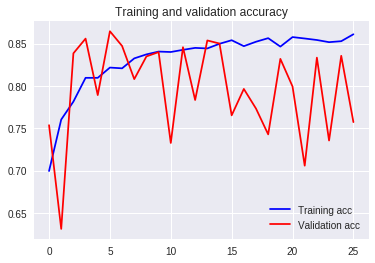
\includegraphics[width=3in,height=2.18in]{mobile/mobilenet-img009.png} 
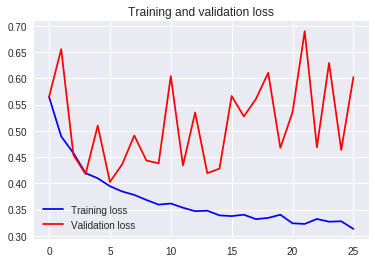
\includegraphics[width=3in,height=2.18in]{mobile/mobilenet-img010.png} 


\begin{table}[ht]
\centering
\caption{Mobilenet Training - Results for Mobilenet + GAP2d + FCN 4096 width + Softmax}
\label{mobilenet1}
\begin{tabular}{rcccl}
\textbf{}   & \textbf{Precision} & \textbf{Recall} & \textbf{F1-Score} & \textbf{Support} \\
No Litter   & 0.97 &0.86 & 0.92 & 1172 \\
Litter      & 0.53 &0.87 & 0.66 & 208 \\
avg / total & 0.91 &0.86 & 0.88 & 1380 \\
\end{tabular}
\begin{center}\noindent\rule{10cm}{0.4pt}\end{center}
\end{table}

\bigskip


\bigskip
\textbf{Mobilenet Conv + Global AveragePooling2D + FCN 2048 width + FCN 2048 width + Softmax Classifier}\newline
Accuracy obtained 0.81884


\bigskip


\bigskip

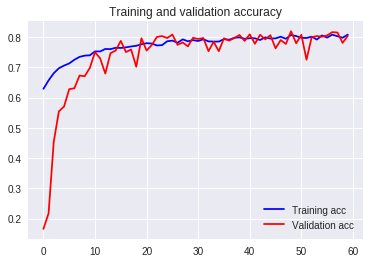
\includegraphics[width=3in,height=2.18in]{mobile/mobilenet-img011.png} 
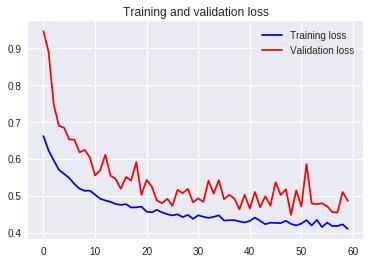
\includegraphics[width=3in,height=2.18in]{mobile/mobilenet-img012.png} 

\begin{table}[ht]
\centering
\caption{Mobilenet Training - Results for Mobilenet + GAP2d + FCN 1024 width + FCN 1024 width + Softmax}
\label{mobilenet1}
\begin{tabular}{rcccl}
\textbf{}   & \textbf{Precision} & \textbf{Recall} & \textbf{F1-Score} & \textbf{Support} \\
No Litter   & 0.97 &0.81 & 0.88 & 1172 \\
Litter      & 0.45 &0.88 & 0.59 & 208 \\
avg / total & 0.89 &0.82 & 0.84 & 1380 \\
\end{tabular}
\begin{center}\noindent\rule{10cm}{0.4pt}\end{center}
\end{table}

\bigskip


\bigskip


\bigskip


\bigskip


\bigskip

\textbf{Mobilenet Conv + Global AveragePooling2D + FCN 1024 width + Softmax Classifier}\newline
\textbf{Mobilenet last conv block (13) trainable 0.9514}

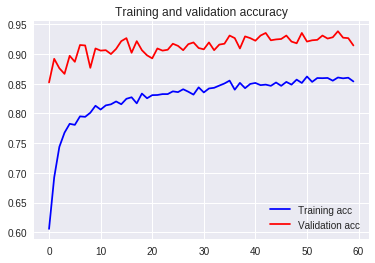
\includegraphics[width=3in,height=2.18in]{mobile/mobilenet-img013.png}
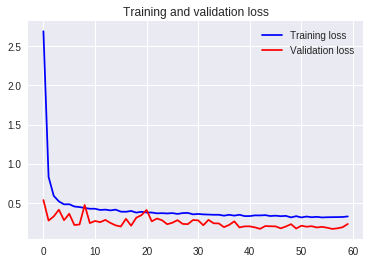
\includegraphics[width=3in,height=2.18in]{mobile/mobilenet-img014.png}


\begin{table}[ht]
\centering
\caption{Mobilenet Training - Results for Mobilenet + GAP2d + FCN 1024 width + Softmax (train conv block 13)}
\label{mobilenet1}
\begin{tabular}{rcccl}
\textbf{}   & \textbf{Precision} & \textbf{Recall} & \textbf{F1-Score} & \textbf{Support} \\
No Litter   & 0.91 &0.99 & 0.95 & 1172 \\
Litter      & 0.94 &0.46 & 0.62 & 208 \\
avg / total & 0.92 &0.91 & 0.90 & 1380 \\
\end{tabular}
\begin{center}\noindent\rule{10cm}{0.4pt}\end{center}
\end{table}

\bigskip

\textbf{Mobilenet last 2 conv block (12 and 13) trainable 0.9514}


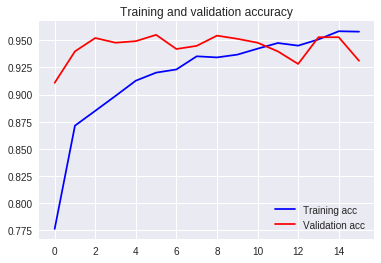
\includegraphics[width=3in,height=2.18in]{mobile/mobilenet-img015.png}
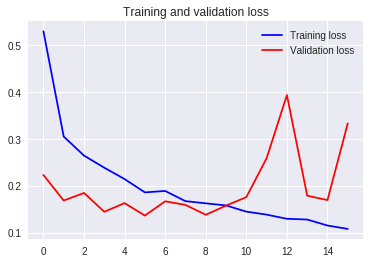
\includegraphics[width=3in,height=2.18in]{mobile/mobilenet-img016.png}


\begin{table}[ht]
\centering
\caption{Mobilenet Training - Results for Mobilenet + GAP2d + FCN 1024 width + Softmax (train conv block 12 and 13}
\label{mobilenet1}
\begin{tabular}{rcccl}
\textbf{}   & \textbf{Precision} & \textbf{Recall} & \textbf{F1-Score} & \textbf{Support} \\
No Litter   & 0.93 &0.99 & 0.96 & 1172 \\
Litter      & 0.95 &0.57 & 0.71 & 208 \\
avg / total & 0.93 &0.93 & 0.92 & 1380 \\
\end{tabular}
\begin{center}\noindent\rule{10cm}{0.4pt}\end{center}
\end{table}

Accuracy improvement stops therefore we assume that layers are already trained.
\cite{Alom2018TheApproaches}
\bibliographystyle{IEEEtran}
\bibliography{mybib}
\end{document}
